
\section{Experiment}
\label{sec:experiments}
To validate the effectiveness of VLA-Cache, we evaluate our method in both simulation and real-world settings. In simulation, we evaluate VLA-Cache on three open-source VLA models: OpenVLA~\cite{kim24openvla}, OpenVLA-OFT~\cite{kim2025fine} and CogAct~\cite{li2024cogact}, using the LIBERO benchmark~\cite{liu2024libero} and SIMPLER environment~\cite{li2024evaluating}, respectively.
All experiments are conducted on an NVIDIA RTX 4090 GPU.

\subsection{Experiment Setup}
\textbf{Compared Methods.} We leverage the architectural similarity between VLA and VLM models, which allows direct application of existing VLM acceleration methods to VLA inference. Specifically, we adopt two state-of-the-art token-level acceleration techniques SparseVLM~\cite{zhang2024sparsevlm} and FastV~\cite{chen2025image} on OpenVLA as compared methods in the LIBERO benchmark.

\textbf{Evaluation Metrics.}
We evaluate VLA-Cache using four metrics: success rate, control frequency, FLOPs, and CUDA latency. Success rate and control frequency respectively assess task performance and the responsiveness of action prediction in closed-loop control. FLOPs measure theoretical computation, while CUDA latency captures actual GPU runtime. These two efficiency metrics are widely adopted in VLM/VLA acceleration methods. 

\subsection{Evaluation Benchmark}  
\textbf{LIBERO.}
The LIBERO Benchmark~\cite{liu2024libero} covers four task suites: Spatial, Object, Goal, and Long, each testing a different aspect of manipulation generalization. We follow the standard setup from OpenVLA~\cite{kim24openvla} and OpenVLA-OFT~\cite{kim2025fine}, using official weights and machines for consistency. Each suite includes ten subtasks evaluated over multiple episodes.

\begin{figure}[!tb]
  \centering
  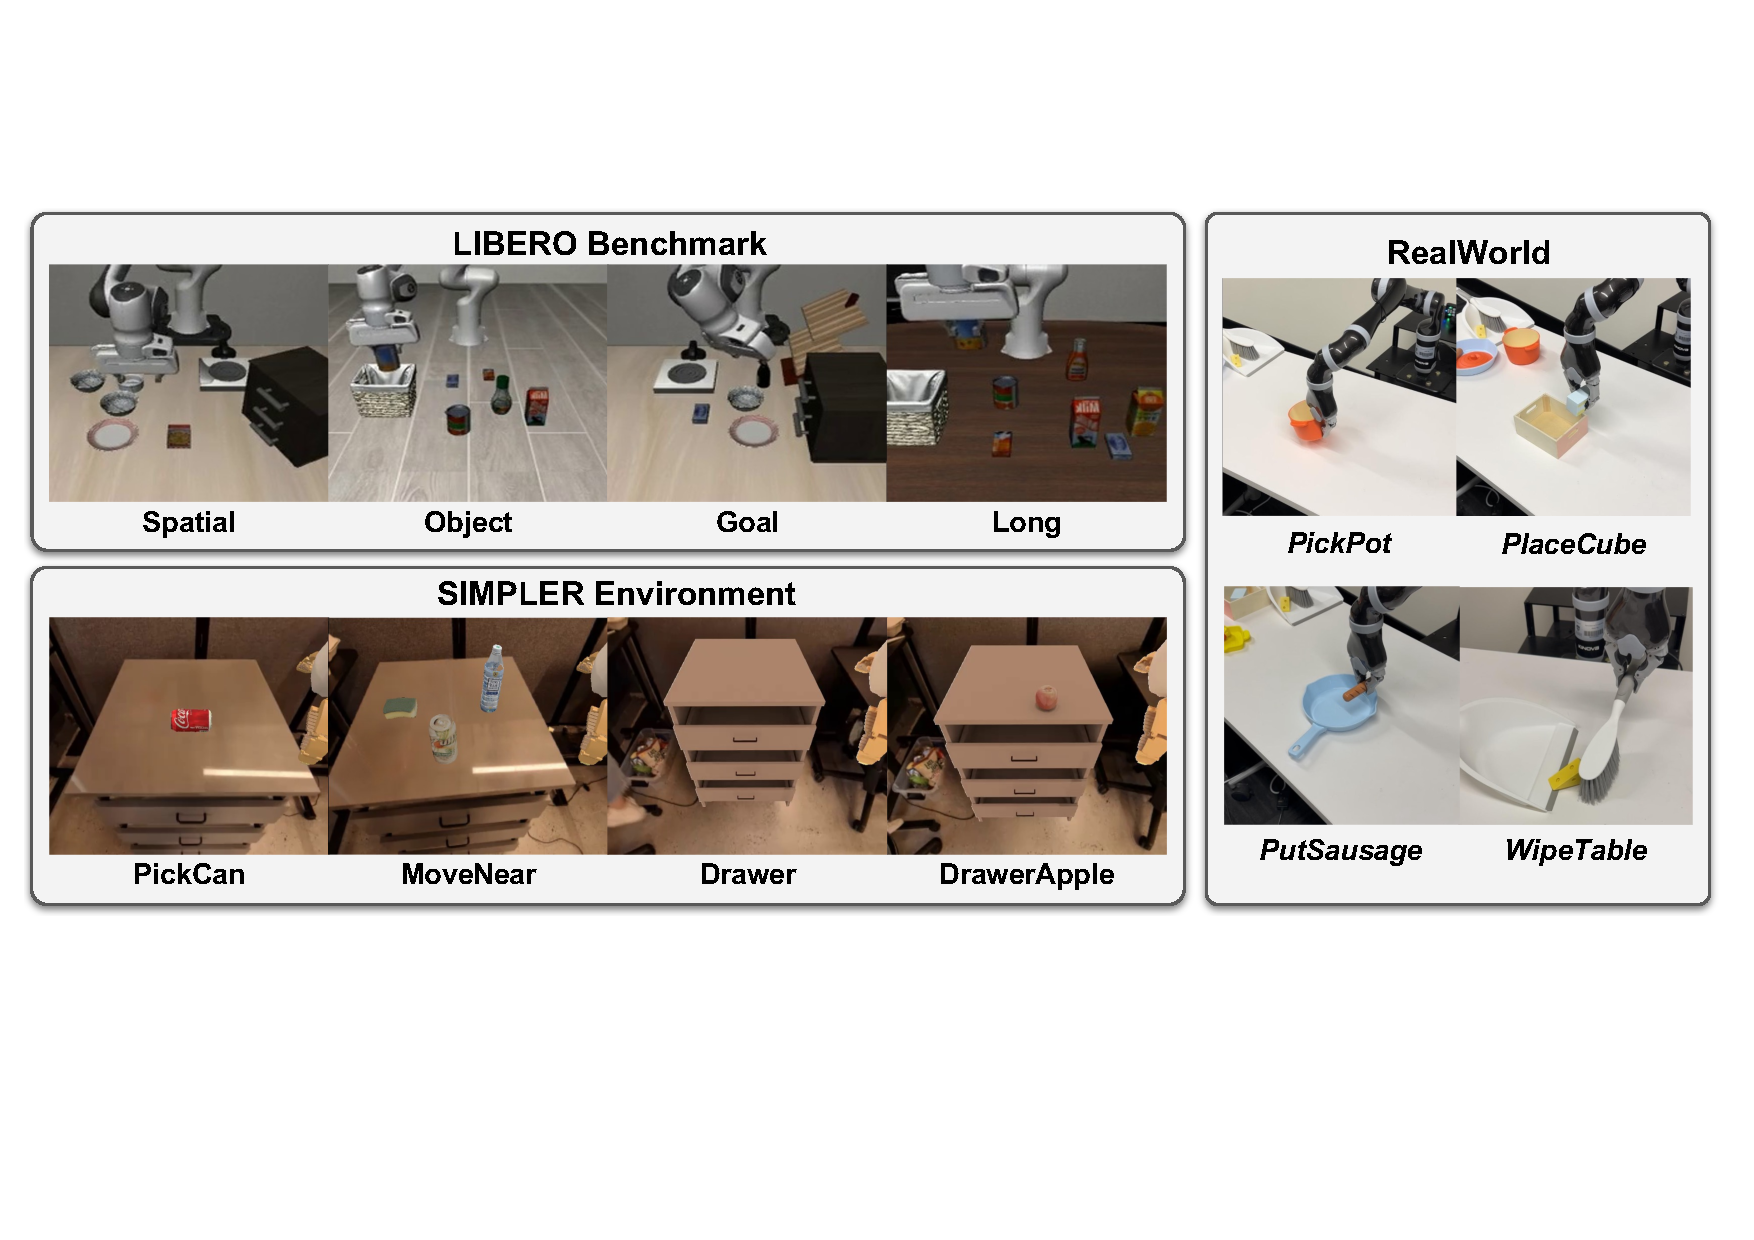
\includegraphics[width=0.9\linewidth]{fig/task_demos.pdf}
  \caption{Tasks on LIBERO Benchmark, the SIMPLER Environment and Real World.}
  \vskip -0.1in
  \label{fig:graph}
\end{figure}

\textbf{SIMPLER.}
The SIMPLER simulator~\cite{li2024evaluating} offers two settings, \emph{Visual Matching} and \emph{Variant Aggregation}, designed to bridge simulation-to-reality gaps. Following CogAct’s setup~\cite{li2024cogact}, we evaluate both settings on a Google robot arm across four manipulation tasks. CogAct, which integrates a Diffusion Policy for continuous control, serves as our baseline. These evaluations demonstrate the generality of VLA-Cache under different action heads and simulation variations.

\textbf{Real Robot Evaluation.}
We deploy VLA-Cache on a Kinova Jaco2 manipulator equipped with a front-facing camera. The robot is evaluated on four tasks: \emph{PickPot}, \emph{PlaceCube}, \emph{PutSausage}, and \emph{WipeTable}, with the last task including diverse distractor objects to test robustness.
Demonstrations are collected via teleoperation at 10\,Hz using an Xbox controller, resulting in 150-200 trajectories per task. We fine-tune OpenVLA with LoRA~\cite{hu2021lora} and evaluate on the same tasks, using the LIBERO tuning setup for consistency. More details about real-world experiments are available in the Appendix\ref{app:realworld_details}.

\subsection{Results on Simulation Environment}

\begin{table*}[t]
\centering
\small
\caption{Comparison of different VLA acceleration methods on the LIBERO benchmark.}
% \resizebox{1\linewidth}{!}{
\vskip -0.05in 
\setlength{\tabcolsep}{2.1mm}{
\begin{tabular}{lcccccccc}
\toprule
\multirow{2}{*}{Method} & \multicolumn{5}{c}{Success Rate $\uparrow$} & \multirow{2}{*}{\shortstack{FLOPs\\(T)$\downarrow$}} & \multirow{2}{*}{\shortstack{Latency\\(ms)$\downarrow$}} & \multirow{2}{*}{\shortstack{Control Freq. \\ (Hz)$\uparrow$}} \\
\cmidrule(lr){2-6}
 & Spatial & Object & Goal & Long & Average &  &  &  \\
\midrule
OpenVLA & \underline{84.4\%} & \underline{86.6\%} & \underline{75.6\%} & \underline{53.2\%} & \underline{75.0\%} & \underline{1.864} & \underline{51.91} & \underline{4.23} \\
 + SparseVLM          & 79.8\% & 67.0\% & 72.6\% & 39.4\% & 64.7\% & 1.407 & 83.39 & 3.72 \\
 + FastV              & 83.4\% & 84.0\% & 74.2\% & 51.6\% & 73.3\% & 1.864 & 53.28 & 4.19 \\
 + \textbf{VLA-Cache} & \textbf{83.8\%} & \textbf{85.8\%} & \textbf{76.4\%} & \textbf{52.8\%} & \textbf{74.7\%} & \textbf{1.355} & \textbf{31.83} & \textbf{4.59} \\
\midrule
OpenVLA-OFT & \underline{97.8\%} & \underline{97.6\%} & \underline{97.6\%} & \underline{94.2\%} & \underline{96.8\%} & \underline{4.013} & \underline{79.05} & \underline{65.10} \\
 + \textbf{VLA-Cache} & \textbf{98.3\%} & 97.5\% & \textbf{98.3\%} & \textbf{95.4\%} & \textbf{97.4\%} & \textbf{3.097} & \textbf{62.59} & \textbf{78.98} \\
\bottomrule
\end{tabular}
}
\vskip -0.05in 
\label{tab:libero_main}
\end{table*}

\begin{table*}[t]
\centering
\caption{Comparison of VLA-Cache within the CogACT model in the SIMPLER environment.}
\vskip -0.05in
\small
\resizebox{\linewidth}{!}{
\begin{tabular}{llcccccccc}
\toprule
\multirow{2}{*}{SIMPLER} & \multirow{2}{*}{Method} 
  & \multicolumn{5}{c}{Success Rate $\uparrow$} 
  & \multirow{2}{*}{\shortstack{FLOPs\\(T)$\downarrow$}} 
  & \multirow{2}{*}{\shortstack{Latency\\(ms) $\downarrow$}} 
  & \multirow{2}{*}{\shortstack{Control Freq. \\ (Hz) $\uparrow$}} \\
\cmidrule(lr){3-7}
& & PickCan & MoveNear & Drawer & DrawerApple & Average & & & \\
\midrule

\multirow{2}{*}{Matching}  
  & CogACT 
    & 91.3\% & \textbf{85.0\%} & \textbf{71.8\%} & 50.9\% & \textbf{74.8\%} 
    & 1.847 
    & 54.29 
    & 12.42 \\
  & \quad + \textbf{VLA-Cache} 
    & \textbf{92.0\%} & 83.3\% & 70.5\% & \textbf{51.6\%} & 74.4\% 
    & \textbf{1.496} 
    & \textbf{39.63} 
    & \textbf{14.66} \\

\midrule

\multirow{2}{*}{Aggregation}  
  & CogACT
    & 89.6\% & 80.8\% & 28.3\% & \textbf{46.6\%} & 61.3\% 
    & 1.807 
    & 53.54 
    & 12.36 \\
  & \quad + \textbf{VLA-Cache}
    & \textbf{91.7\%} & \textbf{79.3\%} & \textbf{32.5\%} & 45.8\% & \textbf{62.3\%} 
    & \textbf{1.493} 
    & \textbf{39.11} 
    & \textbf{14.48} \\

\bottomrule
\end{tabular}
}
\vskip -0.1in
\label{tab:simpler_eval}
\end{table*}


\paragraph{Main Results on LIBERO.}
Table~\ref{tab:libero_main} summarizes results across the four LIBERO task suites. VLA-Cache reduces FLOPs by \textbf{27.31\%} and improves latency by \textbf{1.63$\times$} over standard OpenVLA, with only a 0.3\% drop in success rate. It performs robustly across tasks and exceeds the baseline on goal-oriented manipulation. When applied to OpenVLA-OFT, a faster variant with action chunking, VLA-Cache further boosts control frequency by nearly \textbf{14 Hz}, showing strong compatibility with high-frequency architectures and delivering additive gains even on optimized VLA models. 
In contrast, FastV and SparseVLM fail to improve inference speed and often degrade task performance. Their token pruning and merging strategies operate within a \textit{single frame} and disrupt \textbf{spatial fidelity}, which is critical for precise manipulation. Moreover, these methods target long output sequences, whereas VLA models generate short action outputs (\textit{e.g.}, 7 tokens), rendering the speedups marginal. 
\begin{wraptable}{r}{0.48\textwidth}
\centering
\vskip 0.05in
\caption{Ablation on token pruning/reuse in LIBERO-Spatial using OpenVLA (256 vision tokens). Best values are in \textbf{bold}.}
\small
\resizebox{0.47\textwidth}{!}{ % 缩小内容以适配wraptable宽度
\begin{tabular}{ccccc}
\toprule
\textbf{\#Tokens} & \textbf{Methods} & \textbf{SR \% $\uparrow$} & \textbf{FLOPs $\downarrow$} & \textbf{Latency (ms) $\downarrow$} \\
\midrule
0 & Baseline & 84.4 & 1.888 & 52.37 \\
\midrule
\multirow{3}{*}{50}
  & SparseVLM & 79.8 & \textbf{1.358} & 88.08 \\
  & FastV     & 84.6 & 1.888          & 53.10 \\
  & Ours      & \textbf{85.4} & 1.611 & \textbf{33.43} \\
\midrule
\multirow{3}{*}{100}
  & SparseVLM & 74.6 & \textbf{1.097} & 61.01 \\
  & FastV     & 83.4 & 1.888          & 45.72 \\
  & Ours      & \textbf{83.8} & 1.295 & \textbf{31.29} \\
\midrule
\multirow{3}{*}{200}
  & SparseVLM & 44.4 & \textbf{0.735} & 57.42 \\
  & FastV     & 72.8 & 1.888          & 45.19 \\
  & Ours      & \textbf{68.3} & 0.823 & \textbf{30.29} \\
\bottomrule
\end{tabular}
}
\vskip -0.2in
\label{tab:libero_ablation}
\end{wraptable}



As illustrated in Figure~\ref{fig:sim_visual_redundancy}, VLA-Cache effectively reduces visual computation redundancy during robotic manipulation by precisely identifying static tokens and filtering out task-relevant regions in real time. Notably, OpenVLA-OFT takes both \textit{fixed third-person} and \textit{dynamic wrist-camera} views as inputs. Its strong performance demonstrates that VLA-Cache not only enhances control frequency but also maintains robustness under \textbf{dynamic viewpoints} and camera shifts.

\textbf{Ablation on Token Reusing/Pruning Rate.}
Table~\ref{tab:libero_ablation} presents an ablation study varying the number of reused/pruned tokens. For all methods, aggressive token reduction harms success rate, underscoring the need to preserve informative content. VLA-Cache maintains stable performance at moderate reuse rates (\textit{i.e.}, 100 tokens), while FastV and SparseVLM suffer larger drops due to loss of critical visual details. By directly updating KV entries, VLA-Cache remains more efficient and robust under different token reuse configurations.

\textbf{Token Selection Strategies.}  
As shown in Table~\ref{tab:selection_ablation_inline}, directly reusing all static tokens leads to a notable drop in success rate 74.2\%, indicating that visual similarity alone is insufficient for reliable reuse in robotic control. By filtering out task-relevant tokens based on decoder attention, our method recovers performance to 82.6\%. Introducing a layer-adaptive strategy further improves accuracy to 83.8\%, with minimal increase in CUDA latency. 

\paragraph{Main Results on SIMPLER}
Table~\ref{tab:simpler_eval} indicates that VLA-Cache exhibits success rates comparable to the CogACT baseline in the SIMPLER environment while substantially reducing computational overhead. 

The efficiency gains are evident in the FLOPs and inference time measurements. 
VLA-Cache achieves roughly 20\% fewer FLOPs than the baseline, coupled with a 1.37$\times$ reduction in inference latency. Notably, these results highlight the portability of VLA-Cache across different action heads, establishing it as a general acceleration strategy for VLA. 


\begin{figure*}[!t]
\centering
\vspace{-0.5cm}
{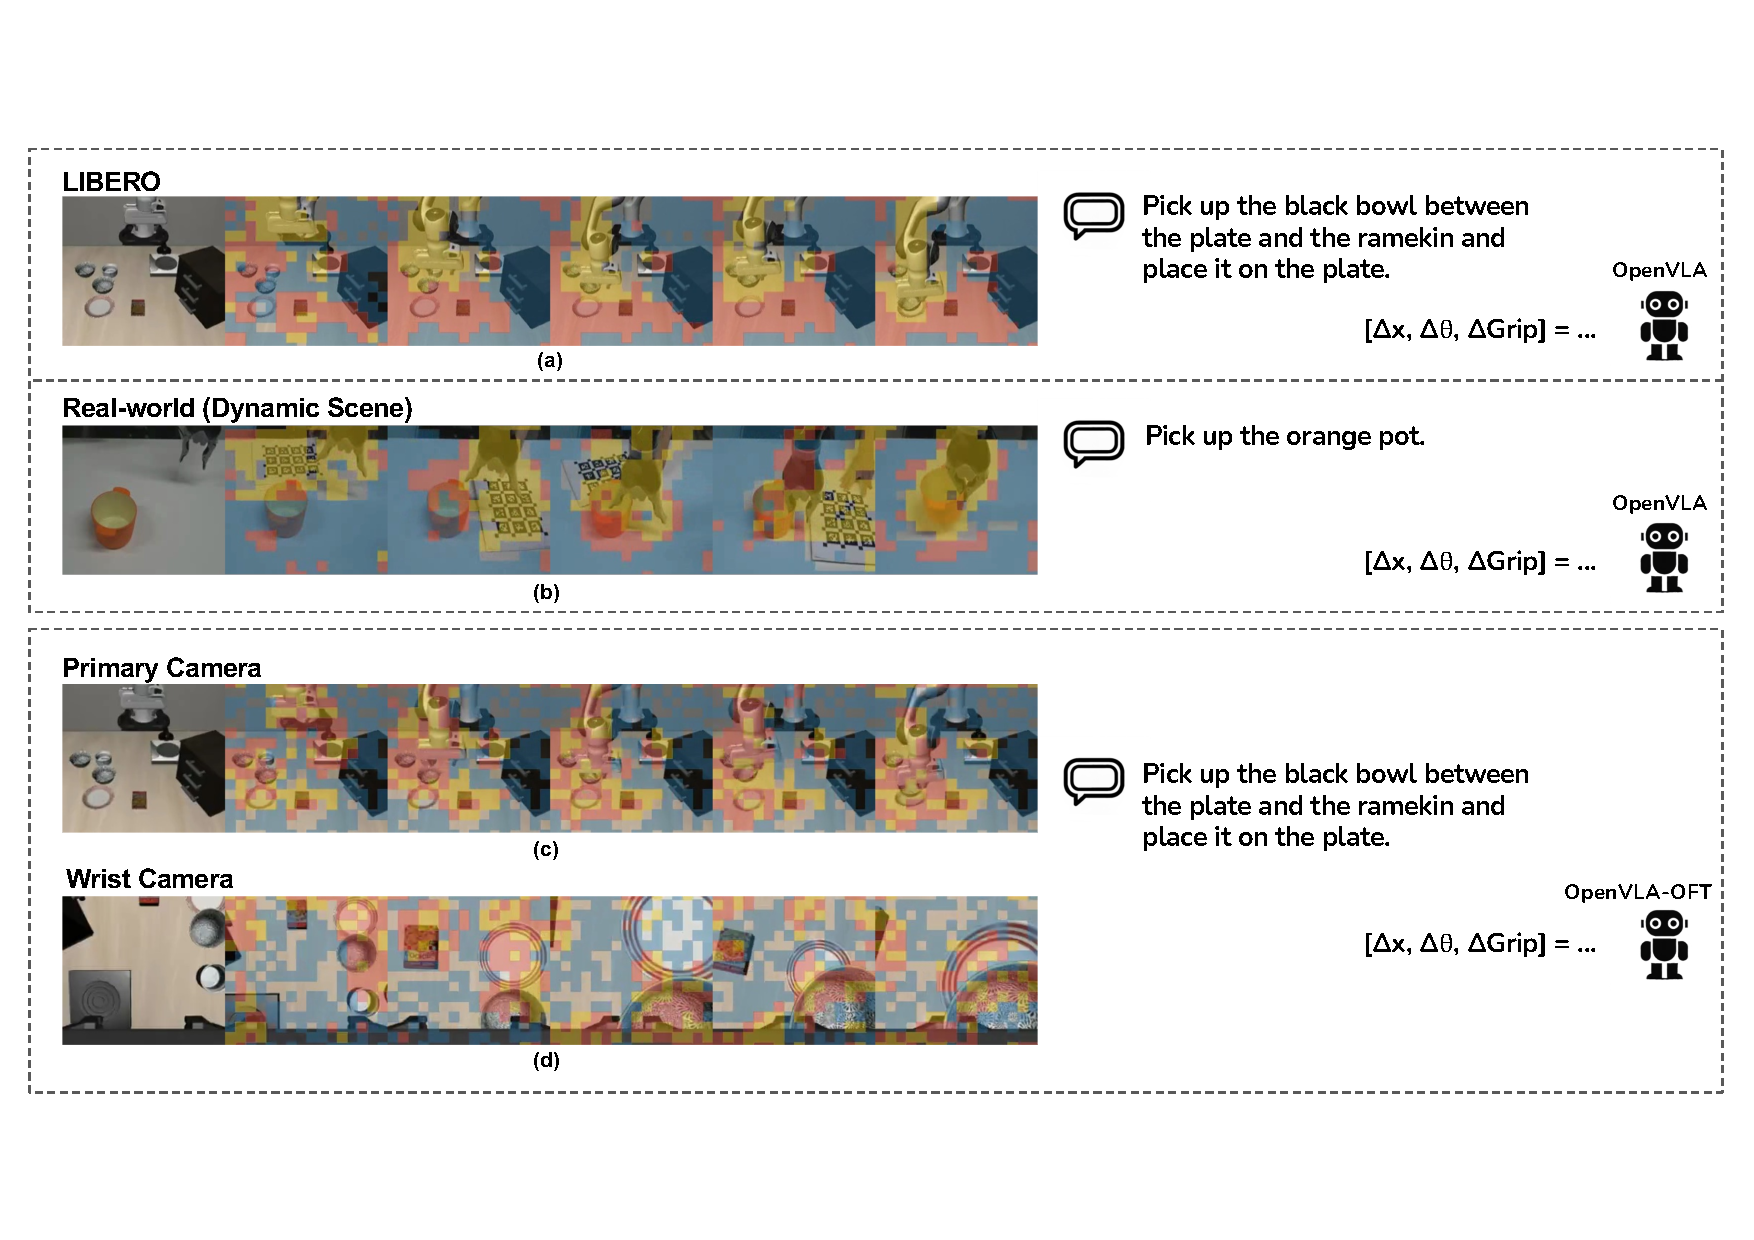
\includegraphics[width=1.0\columnwidth]{fig/simulation_demos.pdf}}
\caption{
Visualization of VLA-Cache token reuse across settings. 
\textbf{(a)} LIBERO simulation with OpenVLA. 
\textbf{(b)} Real-world task under dynamic background. 
\textbf{(c)} and \textbf{(d)} Main and wrist camera views from OpenVLA-OFT. 
\textcolor{blue}{Blue}: static tokens, \textcolor{yellow!70!black}{Yellow}: task-relevant, \textcolor{red}{Red}: overlapping. 
VLA-Cache reduces redundant computation and preserves accuracy under varying conditions.
}
\vskip -0.1in
\label{fig:sim_visual_redundancy}
\end{figure*}

\begin{table*}[!h]
\centering
\caption{Comparison of success rate on real robot tasks.}
\vskip -0.05in
\resizebox{0.98\linewidth}{!}{
\begin{tabular}{lcccccccc}
\toprule
\multirow{2}{*}{Method} 
  & \multicolumn{5}{c}{Success Rate $\uparrow$} 
  & \multirow{2}{*}{\shortstack{FLOPs\\(T)$\downarrow$}} 
  & \multirow{2}{*}{\shortstack{Latency\\(ms) $\downarrow$}} 
  & \multirow{2}{*}{\shortstack{Control Freq. \\ (Hz) $\uparrow$}} \\
\cmidrule(lr){2-6}
& PickPot & PlaceCube & PutSausage & WipeTable & Average & & & \\
\midrule
OpenVLA 
  & \textbf{95.0\%} & 83.3\% & 80.0\% & 70.0\% & 82.1\% 
  & 1.814 & 64.16 & 4.02 \\
 \quad + \textbf{VLA-Cache} 
  & 90.0\% & \textbf{90.0\%} & \textbf{85.0\%} & \textbf{73.3\%} & \textbf{84.6\%} 
  & \textbf{1.303} & \textbf{51.85} & \textbf{4.21} \\
\bottomrule
\end{tabular}
}
\vskip -0.15in
\label{tab:real_robot}
\end{table*}



\subsection{Results on Real Robot}
Table~\ref{tab:real_robot} illustrates the performance of VLA-Cache in real-world robotic tasks. Among the four tasks, \emph{PickPot} shows a slightly lower success rate than the baseline, whereas VLA-Cache exceeds the baseline on other three tasks. The method also achieves considerable reductions in FLOPs and inference time. Overall, VLA-Cache improves the average success rate by 2.4\%, likely due to reduced interference from redundant visual tokens and enhanced decision robustness. With improved robustness as a foundation, VLA-Cache’s ability to prune or reuse redundant tokens may further enhance the model’s resilience, thus yielding higher success rates.

\textbf{Performance under Dynamic Background.}
To assess robustness, we introduced background motion (e.g., human hands and moving objects) in the \emph{PickPot} task. As shown in Table~\ref{tab:real_robot_dynamic}, success rate of baseline dropped from 95\% to 80\% under noise. With VLA-Cache, the same success rate was maintained while reducing FLOPs by 42\% and latency by 35\%. These results highlight VLA-Cache's ability to filter out transient or irrelevant tokens, preserving both efficiency and stability in dynamic real-world settings. Figure~\ref{fig:sim_visual_redundancy} visualizes this effect, showing robust token selection despite background disturbances.
